\chapter{Technical background}\label{chap:theory}

This chapter will address the technical ground inherent to this work.
First comes an overview of Linux operating systems, the distinction between user and kernel mode, and the design of device drivers.

Follow a quick presentation of FPGAs and how they can be driven from the operating system.

\section{Operating system}

%User/kernel space. Networking application: need to send the data through the kernel: huge overhead.

%Crypto API

\subsection{Device Driver}\label{sec:theory-driver}
% General idea of it works
% device driver in userspace: linux userspace i/o (/dev/mem)
Userspace I/O~\cite{koch2011}

There are two ways to get the results from a hardware device: either by using interruption, or by actively polling the device, relentlessly asking it if it finished its operations.
The first case is the cleanest and the most common: when the device has something to send to the driver, or if anything unexpected happened, it sends an interruption request (IRQ) to the processor, which will in turn execute the interruption routine registered by the driver~\citep[chap. 10]{Corbet:2005:LDD:1209083}.
The second case is the easiest and is always guaranteed to work, but won't let go off the processor willingly, loading it at 100\%, and avoiding any other task to be executed.
Hopefully, modern monolithic kernels such as the Linux kernel from 2.6 provide preemptive scheduling~\cite{Santhanam2003}, that is the scheduler interrupts the running task and assigns the processor ressources it used to an other one.
Hence, systems with a lot of processes in need for CPU ressources would not be stalled, but it would not change anything if the only process heavily requesting processor time is the one using the driver.

\section{FPGA}

Driving from the OS: basically, they will need to share some memory.
That memory can be directly mapped and accessed from the user-space using \texttt{/dev/mem}, or can use a direct memory access module (DMA).
From the operation system, we build a bunch of scatterlist in ther kernel-space memory, then map those pages to memory descriptor that have a physical address on the DMA.
They can be mapped three different ways: \texttt{DMA\_BIDIRECTIONAL}, \texttt{DMA\_TO\_DEVICE} or \texttt{DMA\_FROM\_DEVICE}.
When the CPU write something in those descriptor and synchronize them with the DMA, it does not have to care about them anymore, the DMA in now in charge to send them to the device where registers are ready to read the incomming data.
The same goes from the device to the CPU: when the device wants to communicate data to the OS, it writes it on the DMA that will transfer them to the CPU, triggering a flag on the way to notify it.

\section{Cryptography}

\subsection{Symetric cryptography}
Talk about encryption, integrity and authentication.


\subsubsection{AES}
Many modes, CBC is mainly used, GCM is great.

\subsubsection{SHA}
Keyed signature algorithm, several versions in place. SHA-1 is depreciated, SHA-2 is widely used and SHA-3 is already defined and begins to be implemented.

\subsection{Asymetric cryptography}
% Diffie-Hellman: show the math about the shared key, maybe from the course INFOH405 or RFC2631, and point which operation will be offloaded.
Asymetric cryptography relies on a pair of keys: one private known only to the owner of the certificate, and one public available to anyone.
Such cryptography uses two kinds of operations: encryption using the public key of the recipient and digital signature, which is an ecnryption using the private key of the sender.

\subsubsection{RSA}
RSA is a public-key scheme proposed in 1978 by three MIT researchers who gave it their name~\cite{Rivest:1978:MOD:359340.359342}.
A few years later, they founded RSA Laboratories, which is now in charge of maintaining its standards, alongside many others, as the first Public-Key Cryptography Standards, \textit{aka} PKCS \#1.
The last version of the standard is the version 2.2~\cite{pkcs1} and is defined as a precise key generation protocol allowing encryption and decryption.
The keys can be generated by respecting a few steps:
\begin{enumerate}
	\item randomy choose two large primes $p$ and $q$;
	\item compute the modulus $n = p q$, and consequently we have $\phi(n) = (p-1)(q-1)$, with $\phi(n)$ as the Euler function;
	\item randomly choose the public exponent $e \in ]1,\phi(n)[\ s.t.\ GCD(e,\phi(n)) = 1$;
	\item compute $d \in ]1,\phi(n)[\ s.t.\ e \cdot d \equiv 1 (mod\ \phi(n))$
\end{enumerate}

With those parameters, we can form a public key with the pair $(n, e)$ and a private key with the pair $(n, d)$.

The encryption and decryption of a given message $m \in \mathds{Z}_n$ are defined as follows:
\begin{description}
	\item[Encryption] $c = m^e\ mod\ n$
	\item[Decryption] $m = c^d\ mod\ n$
\end{description}




\subsubsection{Diffie-Hellman}
Diffie-Hellman is a secret key exchange protocol: two parties compute a shared secret $ZZ$ that can be used as a symetric key during the following exchanges.
It uses the same kind of operation as RSA, that is modular exponentiation.
The protocol can be one of two type (\cite{rfc2631}, \cite{Frankel:2005:SGI:2206289}):
\begin{itemize}
	\item Static: the actors use their authenticated certificate to compute the shared secret.
	\item Ephemeral: the actors create a new pair of public/private keys from which the secret key is derived.
	\item Anonymous: same as ephemeral, but without signing anything, hence not identifying neither of the actors. This mode is not advisable since it's vulnerable to main-in-the-middle attack.
\end{itemize}
A static scheme is easier to implement and requires much less operations, but using ephemeral keys is essential to ensure perfect forward secrecy.
Imagine that somehow, an opponent lays his hand on the shared secret.
If that secret has already been used, he can decipher all data transfered during past connections.
However, if the secret is new for every new connection, the compromission of the shared secret des not jeopardize past communications.
This is perfect forward secrecy: using a new key to protect the past.

Hereunder is the generation of an ephemeral shared secret.
For a static secret, Alice and Bob will simply use their static certificate, sparing the modular exponentiation of the ephemeral public key generation.
\begin{enumerate}
	\item Alice generates once $p$ and $g$ (using precomputed parameters):
	\begin{description}[nosep]
		\item[p] large prime number
		\item[g] a generator of $\mathds{Z}_p^*$
	\end{description}
	\item Alice picks a random integer $x_a$ and computes $g^{x_a} mod\ p = y_a$.
	\item Alice sends $p$, $g$ and $y_a$ to Bob, signing everything using her private certificate.
	\item Bob checks the signature and picks $x_b$.
	\item Bob computes $y_a^{x_b} mod\ p = g^{x_a x_b} mod\ p = ZZ$, the shared secret to use as a premaster key from which will be derived the symetric key for further communications.
	\item Bob sends $y_b = g^{x_b} mod\ p$, signing everything with his private certificate.
	\item Alice checks the signature and computes the same shared secret: $ZZ = y_b^{x_a} mod\ p = g^{x_a x_b} mod\ p$
\end{enumerate}

If the server is Alice, it has to do at least one signature, one signature verification and two modular exponentiations.
Note that the client, B in our case, could have one signature less because RFC 5246~\cite{rfc5246} leave it as an optional feature, and the server would then have one verification less.
However, any sane configuration will have both actors signing their ephemeral public key.
If the certificate use RSA, we end up with four modular exponentiations, which can become quite heavy computing wise for certain sizes of prime numbers.
We will see in chapter~\ref{chap:results} that while a 1024-bit prime is easily manageable by full software implementation, hardware offloading become a necessity for 4096-bit primes.
Moreover, 1024-bit parameter size, both RSA and Diffie-Hellman, are disallowed by the NIST recommandations since 2013~\cite{nist-sp800-131A}.

\section{Network and VPN implementation}

% Present the TCP/IP layering

% First explain what a VPN is.

There exist several major implementations of VPN: SSL, IPSec and PPTP.
The later was developped by a vendor consortium and proposed in the RFC 2637 and will not be discussed further.

\subsection{SSL/TLS}
% Introduce SSL/TLS, talk about the protocol, the key exchange and stuff, but leaver OpenVPN for the 'implementation' chapter.
% Question the security? Apparently, it does mac-then-encrypt, which is insecure regarding certain types of attacks \cite{cryptoeprint:2001:045}.
% Plus, SSLv3 is to be deprecated, according to a queued RFC: http://www.rfc-editor.org/internet-drafts/draft-ietf-tls-sslv3-diediedie-03.txt

\subsection{IPSec}
% IPSec as a protocol, strongswan come in the 'implementation' chapter.

\begin{figure}[ht]
\center
\subfloat[\label{fig:ipsec-transport}Transport]{%
	\large
	\resizebox{.465\linewidth}{!}{%
	% Graphic for TeX using PGF
% Title: /home/para/documents/polytech2015/MA2/Master_thesis/master_thesis/ipsec-transport.dia
% Creator: Dia v0.97.3
% CreationDate: Thu May 21 00:33:06 2015
% For: para
% \usepackage{tikz}
% The following commands are not supported in PSTricks at present
% We define them conditionally, so when they are implemented,
% this pgf file will use them.
\ifx\du\undefined
  \newlength{\du}
\fi
\setlength{\du}{15\unitlength}
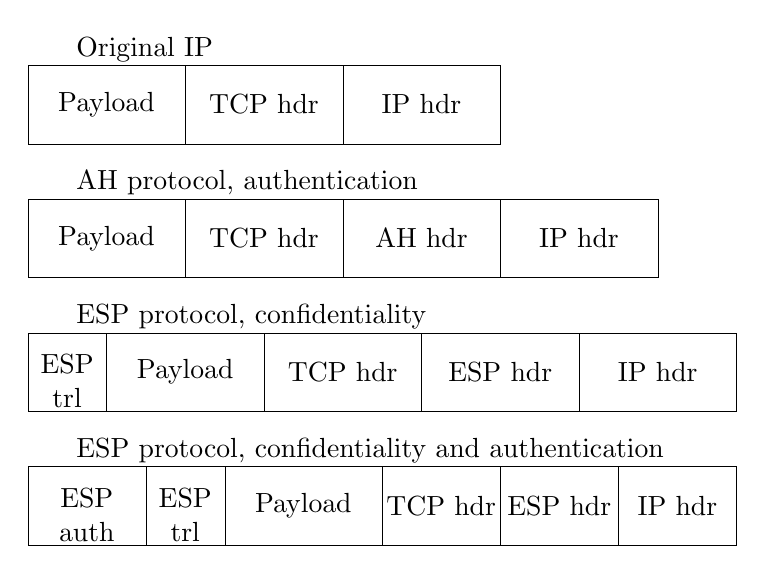
\begin{tikzpicture}
\pgftransformxscale{1.000000}
\pgftransformyscale{-1.000000}
\definecolor{dialinecolor}{rgb}{0.000000, 0.000000, 0.000000}
\pgfsetstrokecolor{dialinecolor}
\definecolor{dialinecolor}{rgb}{1.000000, 1.000000, 1.000000}
\pgfsetfillcolor{dialinecolor}
\pgfsetlinewidth{0.050000\du}
\pgfsetdash{}{0pt}
\pgfsetdash{}{0pt}
\pgfsetmiterjoin
\definecolor{dialinecolor}{rgb}{1.000000, 1.000000, 1.000000}
\pgfsetfillcolor{dialinecolor}
\fill (17.500000\du,15.100000\du)--(17.500000\du,16.100000\du)--(19.000000\du,16.100000\du)--(19.000000\du,15.100000\du)--cycle;
\definecolor{dialinecolor}{rgb}{0.000000, 0.000000, 0.000000}
\pgfsetstrokecolor{dialinecolor}
\draw (17.500000\du,15.100000\du)--(17.500000\du,16.100000\du)--(19.000000\du,16.100000\du)--(19.000000\du,15.100000\du)--cycle;
\pgfsetlinewidth{0.050000\du}
\pgfsetdash{}{0pt}
\pgfsetdash{}{0pt}
\pgfsetmiterjoin
\definecolor{dialinecolor}{rgb}{1.000000, 1.000000, 1.000000}
\pgfsetfillcolor{dialinecolor}
\fill (17.000000\du,13.400000\du)--(17.000000\du,14.400000\du)--(19.000000\du,14.400000\du)--(19.000000\du,13.400000\du)--cycle;
\definecolor{dialinecolor}{rgb}{0.000000, 0.000000, 0.000000}
\pgfsetstrokecolor{dialinecolor}
\draw (17.000000\du,13.400000\du)--(17.000000\du,14.400000\du)--(19.000000\du,14.400000\du)--(19.000000\du,13.400000\du)--cycle;
\pgfsetlinewidth{0.050000\du}
\pgfsetdash{}{0pt}
\pgfsetdash{}{0pt}
\pgfsetmiterjoin
\definecolor{dialinecolor}{rgb}{1.000000, 1.000000, 1.000000}
\pgfsetfillcolor{dialinecolor}
\fill (16.000000\du,11.700000\du)--(16.000000\du,12.700000\du)--(18.000000\du,12.700000\du)--(18.000000\du,11.700000\du)--cycle;
\definecolor{dialinecolor}{rgb}{0.000000, 0.000000, 0.000000}
\pgfsetstrokecolor{dialinecolor}
\draw (16.000000\du,11.700000\du)--(16.000000\du,12.700000\du)--(18.000000\du,12.700000\du)--(18.000000\du,11.700000\du)--cycle;
\pgfsetlinewidth{0.050000\du}
\pgfsetdash{}{0pt}
\pgfsetdash{}{0pt}
\pgfsetmiterjoin
\definecolor{dialinecolor}{rgb}{1.000000, 1.000000, 1.000000}
\pgfsetfillcolor{dialinecolor}
\fill (14.000000\du,10.000000\du)--(14.000000\du,11.000000\du)--(16.000000\du,11.000000\du)--(16.000000\du,10.000000\du)--cycle;
\definecolor{dialinecolor}{rgb}{0.000000, 0.000000, 0.000000}
\pgfsetstrokecolor{dialinecolor}
\draw (14.000000\du,10.000000\du)--(14.000000\du,11.000000\du)--(16.000000\du,11.000000\du)--(16.000000\du,10.000000\du)--cycle;
\pgfsetlinewidth{0.050000\du}
\pgfsetdash{}{0pt}
\pgfsetdash{}{0pt}
\pgfsetmiterjoin
\definecolor{dialinecolor}{rgb}{1.000000, 1.000000, 1.000000}
\pgfsetfillcolor{dialinecolor}
\fill (10.000000\du,10.000000\du)--(10.000000\du,11.000000\du)--(12.000000\du,11.000000\du)--(12.000000\du,10.000000\du)--cycle;
\definecolor{dialinecolor}{rgb}{0.000000, 0.000000, 0.000000}
\pgfsetstrokecolor{dialinecolor}
\draw (10.000000\du,10.000000\du)--(10.000000\du,11.000000\du)--(12.000000\du,11.000000\du)--(12.000000\du,10.000000\du)--cycle;
% setfont left to latex
\definecolor{dialinecolor}{rgb}{0.000000, 0.000000, 0.000000}
\pgfsetstrokecolor{dialinecolor}
\node at (11.000000\du,10.500000\du){Payload};
\pgfsetlinewidth{0.050000\du}
\pgfsetdash{}{0pt}
\pgfsetdash{}{0pt}
\pgfsetmiterjoin
\definecolor{dialinecolor}{rgb}{1.000000, 1.000000, 1.000000}
\pgfsetfillcolor{dialinecolor}
\fill (12.000000\du,10.000000\du)--(12.000000\du,11.000000\du)--(14.000000\du,11.000000\du)--(14.000000\du,10.000000\du)--cycle;
\definecolor{dialinecolor}{rgb}{0.000000, 0.000000, 0.000000}
\pgfsetstrokecolor{dialinecolor}
\draw (12.000000\du,10.000000\du)--(12.000000\du,11.000000\du)--(14.000000\du,11.000000\du)--(14.000000\du,10.000000\du)--cycle;
% setfont left to latex
\definecolor{dialinecolor}{rgb}{0.000000, 0.000000, 0.000000}
\pgfsetstrokecolor{dialinecolor}
\node at (15.000000\du,10.500000\du){IP hdr};
% setfont left to latex
\definecolor{dialinecolor}{rgb}{0.000000, 0.000000, 0.000000}
\pgfsetstrokecolor{dialinecolor}
\node at (13.000000\du,10.500000\du){TCP hdr};
\pgfsetlinewidth{0.050000\du}
\pgfsetdash{}{0pt}
\pgfsetdash{}{0pt}
\pgfsetmiterjoin
\definecolor{dialinecolor}{rgb}{1.000000, 1.000000, 1.000000}
\pgfsetfillcolor{dialinecolor}
\fill (10.000000\du,11.700000\du)--(10.000000\du,12.700000\du)--(12.000000\du,12.700000\du)--(12.000000\du,11.700000\du)--cycle;
\definecolor{dialinecolor}{rgb}{0.000000, 0.000000, 0.000000}
\pgfsetstrokecolor{dialinecolor}
\draw (10.000000\du,11.700000\du)--(10.000000\du,12.700000\du)--(12.000000\du,12.700000\du)--(12.000000\du,11.700000\du)--cycle;
% setfont left to latex
\definecolor{dialinecolor}{rgb}{0.000000, 0.000000, 0.000000}
\pgfsetstrokecolor{dialinecolor}
\node at (11.000000\du,12.200000\du){Payload};
\pgfsetlinewidth{0.050000\du}
\pgfsetdash{}{0pt}
\pgfsetdash{}{0pt}
\pgfsetmiterjoin
\definecolor{dialinecolor}{rgb}{1.000000, 1.000000, 1.000000}
\pgfsetfillcolor{dialinecolor}
\fill (12.000000\du,11.700000\du)--(12.000000\du,12.700000\du)--(14.000000\du,12.700000\du)--(14.000000\du,11.700000\du)--cycle;
\definecolor{dialinecolor}{rgb}{0.000000, 0.000000, 0.000000}
\pgfsetstrokecolor{dialinecolor}
\draw (12.000000\du,11.700000\du)--(12.000000\du,12.700000\du)--(14.000000\du,12.700000\du)--(14.000000\du,11.700000\du)--cycle;
% setfont left to latex
\definecolor{dialinecolor}{rgb}{0.000000, 0.000000, 0.000000}
\pgfsetstrokecolor{dialinecolor}
\node at (17.000000\du,12.200000\du){IP hdr};
% setfont left to latex
\definecolor{dialinecolor}{rgb}{0.000000, 0.000000, 0.000000}
\pgfsetstrokecolor{dialinecolor}
\node at (13.000000\du,12.200000\du){TCP hdr};
\pgfsetlinewidth{0.050000\du}
\pgfsetdash{}{0pt}
\pgfsetdash{}{0pt}
\pgfsetmiterjoin
\definecolor{dialinecolor}{rgb}{1.000000, 1.000000, 1.000000}
\pgfsetfillcolor{dialinecolor}
\fill (14.000000\du,11.700000\du)--(14.000000\du,12.700000\du)--(16.000000\du,12.700000\du)--(16.000000\du,11.700000\du)--cycle;
\definecolor{dialinecolor}{rgb}{0.000000, 0.000000, 0.000000}
\pgfsetstrokecolor{dialinecolor}
\draw (14.000000\du,11.700000\du)--(14.000000\du,12.700000\du)--(16.000000\du,12.700000\du)--(16.000000\du,11.700000\du)--cycle;
% setfont left to latex
\definecolor{dialinecolor}{rgb}{0.000000, 0.000000, 0.000000}
\pgfsetstrokecolor{dialinecolor}
\node at (15.000000\du,12.200000\du){AH hdr};
% setfont left to latex
\definecolor{dialinecolor}{rgb}{0.000000, 0.000000, 0.000000}
\pgfsetstrokecolor{dialinecolor}
\node[anchor=west] at (10.500000\du,9.800000\du){Original IP};
% setfont left to latex
\definecolor{dialinecolor}{rgb}{0.000000, 0.000000, 0.000000}
\pgfsetstrokecolor{dialinecolor}
\node[anchor=west] at (10.500000\du,11.500000\du){AH protocol, authentication};
\pgfsetlinewidth{0.050000\du}
\pgfsetdash{}{0pt}
\pgfsetdash{}{0pt}
\pgfsetmiterjoin
\definecolor{dialinecolor}{rgb}{1.000000, 1.000000, 1.000000}
\pgfsetfillcolor{dialinecolor}
\fill (11.000000\du,13.400000\du)--(11.000000\du,14.400000\du)--(13.000000\du,14.400000\du)--(13.000000\du,13.400000\du)--cycle;
\definecolor{dialinecolor}{rgb}{0.000000, 0.000000, 0.000000}
\pgfsetstrokecolor{dialinecolor}
\draw (11.000000\du,13.400000\du)--(11.000000\du,14.400000\du)--(13.000000\du,14.400000\du)--(13.000000\du,13.400000\du)--cycle;
% setfont left to latex
\definecolor{dialinecolor}{rgb}{0.000000, 0.000000, 0.000000}
\pgfsetstrokecolor{dialinecolor}
\node at (12.000000\du,13.900000\du){Payload};
\pgfsetlinewidth{0.050000\du}
\pgfsetdash{}{0pt}
\pgfsetdash{}{0pt}
\pgfsetmiterjoin
\definecolor{dialinecolor}{rgb}{1.000000, 1.000000, 1.000000}
\pgfsetfillcolor{dialinecolor}
\fill (13.000000\du,13.400000\du)--(13.000000\du,14.400000\du)--(15.000000\du,14.400000\du)--(15.000000\du,13.400000\du)--cycle;
\definecolor{dialinecolor}{rgb}{0.000000, 0.000000, 0.000000}
\pgfsetstrokecolor{dialinecolor}
\draw (13.000000\du,13.400000\du)--(13.000000\du,14.400000\du)--(15.000000\du,14.400000\du)--(15.000000\du,13.400000\du)--cycle;
% setfont left to latex
\definecolor{dialinecolor}{rgb}{0.000000, 0.000000, 0.000000}
\pgfsetstrokecolor{dialinecolor}
\node at (18.000000\du,13.900000\du){IP hdr};
% setfont left to latex
\definecolor{dialinecolor}{rgb}{0.000000, 0.000000, 0.000000}
\pgfsetstrokecolor{dialinecolor}
\node at (14.000000\du,13.900000\du){TCP hdr};
\pgfsetlinewidth{0.050000\du}
\pgfsetdash{}{0pt}
\pgfsetdash{}{0pt}
\pgfsetmiterjoin
\definecolor{dialinecolor}{rgb}{1.000000, 1.000000, 1.000000}
\pgfsetfillcolor{dialinecolor}
\fill (15.000000\du,13.400000\du)--(15.000000\du,14.400000\du)--(17.000000\du,14.400000\du)--(17.000000\du,13.400000\du)--cycle;
\definecolor{dialinecolor}{rgb}{0.000000, 0.000000, 0.000000}
\pgfsetstrokecolor{dialinecolor}
\draw (15.000000\du,13.400000\du)--(15.000000\du,14.400000\du)--(17.000000\du,14.400000\du)--(17.000000\du,13.400000\du)--cycle;
% setfont left to latex
\definecolor{dialinecolor}{rgb}{0.000000, 0.000000, 0.000000}
\pgfsetstrokecolor{dialinecolor}
\node at (16.000000\du,13.900000\du){ESP hdr};
\pgfsetlinewidth{0.050000\du}
\pgfsetdash{}{0pt}
\pgfsetdash{}{0pt}
\pgfsetmiterjoin
\definecolor{dialinecolor}{rgb}{1.000000, 1.000000, 1.000000}
\pgfsetfillcolor{dialinecolor}
\fill (10.000000\du,13.400000\du)--(10.000000\du,14.400000\du)--(11.000000\du,14.400000\du)--(11.000000\du,13.400000\du)--cycle;
\definecolor{dialinecolor}{rgb}{0.000000, 0.000000, 0.000000}
\pgfsetstrokecolor{dialinecolor}
\draw (10.000000\du,13.400000\du)--(10.000000\du,14.400000\du)--(11.000000\du,14.400000\du)--(11.000000\du,13.400000\du)--cycle;
% setfont left to latex
\definecolor{dialinecolor}{rgb}{0.000000, 0.000000, 0.000000}
\pgfsetstrokecolor{dialinecolor}
\node at (10.500000\du,13.804583\du){ESP};
% setfont left to latex
\definecolor{dialinecolor}{rgb}{0.000000, 0.000000, 0.000000}
\pgfsetstrokecolor{dialinecolor}
\node at (10.500000\du,14.227917\du){trl};
% setfont left to latex
\definecolor{dialinecolor}{rgb}{0.000000, 0.000000, 0.000000}
\pgfsetstrokecolor{dialinecolor}
\node[anchor=west] at (10.500000\du,13.200000\du){ESP protocol, confidentiality};
\pgfsetlinewidth{0.050000\du}
\pgfsetdash{}{0pt}
\pgfsetdash{}{0pt}
\pgfsetmiterjoin
\definecolor{dialinecolor}{rgb}{1.000000, 1.000000, 1.000000}
\pgfsetfillcolor{dialinecolor}
\fill (12.500000\du,15.100000\du)--(12.500000\du,16.100000\du)--(14.500000\du,16.100000\du)--(14.500000\du,15.100000\du)--cycle;
\definecolor{dialinecolor}{rgb}{0.000000, 0.000000, 0.000000}
\pgfsetstrokecolor{dialinecolor}
\draw (12.500000\du,15.100000\du)--(12.500000\du,16.100000\du)--(14.500000\du,16.100000\du)--(14.500000\du,15.100000\du)--cycle;
% setfont left to latex
\definecolor{dialinecolor}{rgb}{0.000000, 0.000000, 0.000000}
\pgfsetstrokecolor{dialinecolor}
\node at (13.500000\du,15.600000\du){Payload};
\pgfsetlinewidth{0.050000\du}
\pgfsetdash{}{0pt}
\pgfsetdash{}{0pt}
\pgfsetmiterjoin
\definecolor{dialinecolor}{rgb}{1.000000, 1.000000, 1.000000}
\pgfsetfillcolor{dialinecolor}
\fill (14.500000\du,15.100000\du)--(14.500000\du,16.100000\du)--(16.000000\du,16.100000\du)--(16.000000\du,15.100000\du)--cycle;
\definecolor{dialinecolor}{rgb}{0.000000, 0.000000, 0.000000}
\pgfsetstrokecolor{dialinecolor}
\draw (14.500000\du,15.100000\du)--(14.500000\du,16.100000\du)--(16.000000\du,16.100000\du)--(16.000000\du,15.100000\du)--cycle;
% setfont left to latex
\definecolor{dialinecolor}{rgb}{0.000000, 0.000000, 0.000000}
\pgfsetstrokecolor{dialinecolor}
\node at (18.250000\du,15.600000\du){IP hdr};
% setfont left to latex
\definecolor{dialinecolor}{rgb}{0.000000, 0.000000, 0.000000}
\pgfsetstrokecolor{dialinecolor}
\node at (15.250000\du,15.600000\du){TCP hdr};
\pgfsetlinewidth{0.050000\du}
\pgfsetdash{}{0pt}
\pgfsetdash{}{0pt}
\pgfsetmiterjoin
\definecolor{dialinecolor}{rgb}{1.000000, 1.000000, 1.000000}
\pgfsetfillcolor{dialinecolor}
\fill (16.000000\du,15.100000\du)--(16.000000\du,16.100000\du)--(17.500000\du,16.100000\du)--(17.500000\du,15.100000\du)--cycle;
\definecolor{dialinecolor}{rgb}{0.000000, 0.000000, 0.000000}
\pgfsetstrokecolor{dialinecolor}
\draw (16.000000\du,15.100000\du)--(16.000000\du,16.100000\du)--(17.500000\du,16.100000\du)--(17.500000\du,15.100000\du)--cycle;
% setfont left to latex
\definecolor{dialinecolor}{rgb}{0.000000, 0.000000, 0.000000}
\pgfsetstrokecolor{dialinecolor}
\node at (16.750000\du,15.600000\du){ESP hdr};
\pgfsetlinewidth{0.050000\du}
\pgfsetdash{}{0pt}
\pgfsetdash{}{0pt}
\pgfsetmiterjoin
\definecolor{dialinecolor}{rgb}{1.000000, 1.000000, 1.000000}
\pgfsetfillcolor{dialinecolor}
\fill (11.500000\du,15.100000\du)--(11.500000\du,16.100000\du)--(12.500000\du,16.100000\du)--(12.500000\du,15.100000\du)--cycle;
\definecolor{dialinecolor}{rgb}{0.000000, 0.000000, 0.000000}
\pgfsetstrokecolor{dialinecolor}
\draw (11.500000\du,15.100000\du)--(11.500000\du,16.100000\du)--(12.500000\du,16.100000\du)--(12.500000\du,15.100000\du)--cycle;
% setfont left to latex
\definecolor{dialinecolor}{rgb}{0.000000, 0.000000, 0.000000}
\pgfsetstrokecolor{dialinecolor}
\node at (12.000000\du,15.504583\du){ESP};
% setfont left to latex
\definecolor{dialinecolor}{rgb}{0.000000, 0.000000, 0.000000}
\pgfsetstrokecolor{dialinecolor}
\node at (12.000000\du,15.927917\du){trl};
\pgfsetlinewidth{0.050000\du}
\pgfsetdash{}{0pt}
\pgfsetdash{}{0pt}
\pgfsetmiterjoin
\definecolor{dialinecolor}{rgb}{1.000000, 1.000000, 1.000000}
\pgfsetfillcolor{dialinecolor}
\fill (10.000000\du,15.100000\du)--(10.000000\du,16.100000\du)--(11.500000\du,16.100000\du)--(11.500000\du,15.100000\du)--cycle;
\definecolor{dialinecolor}{rgb}{0.000000, 0.000000, 0.000000}
\pgfsetstrokecolor{dialinecolor}
\draw (10.000000\du,15.100000\du)--(10.000000\du,16.100000\du)--(11.500000\du,16.100000\du)--(11.500000\du,15.100000\du)--cycle;
% setfont left to latex
\definecolor{dialinecolor}{rgb}{0.000000, 0.000000, 0.000000}
\pgfsetstrokecolor{dialinecolor}
\node at (10.750000\du,15.504583\du){ESP};
% setfont left to latex
\definecolor{dialinecolor}{rgb}{0.000000, 0.000000, 0.000000}
\pgfsetstrokecolor{dialinecolor}
\node at (10.750000\du,15.927917\du){auth};
% setfont left to latex
\definecolor{dialinecolor}{rgb}{0.000000, 0.000000, 0.000000}
\pgfsetstrokecolor{dialinecolor}
\node[anchor=west] at (10.500000\du,14.900000\du){ESP protocol, confidentiality and authentication};
\end{tikzpicture}

	}
}
\subfloat[\label{fig:ipsec-tunnel}Tunnel]{%
	\large
	\resizebox{.535\linewidth}{!}{%
	% Graphic for TeX using PGF
% Title: /home/para/ipsec-tunnel.dia
% Creator: Dia v0.97.3
% CreationDate: Thu May 21 00:36:17 2015
% For: para
% \usepackage{tikz}
% The following commands are not supported in PSTricks at present
% We define them conditionally, so when they are implemented,
% this pgf file will use them.
\ifx\du\undefined
  \newlength{\du}
\fi
\setlength{\du}{15\unitlength}
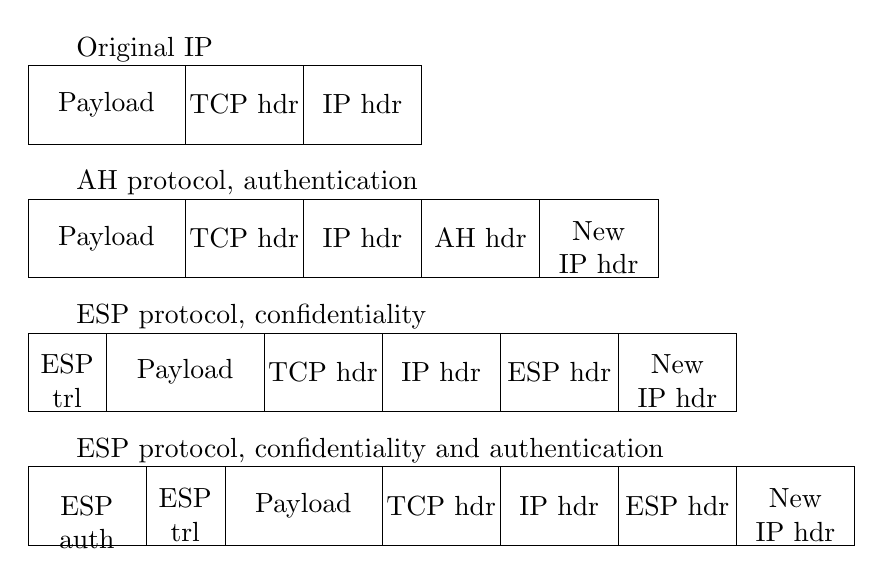
\begin{tikzpicture}
\pgftransformxscale{1.000000}
\pgftransformyscale{-1.000000}
\definecolor{dialinecolor}{rgb}{0.000000, 0.000000, 0.000000}
\pgfsetstrokecolor{dialinecolor}
\definecolor{dialinecolor}{rgb}{1.000000, 1.000000, 1.000000}
\pgfsetfillcolor{dialinecolor}
\pgfsetlinewidth{0.050000\du}
\pgfsetdash{}{0pt}
\pgfsetdash{}{0pt}
\pgfsetmiterjoin
\definecolor{dialinecolor}{rgb}{1.000000, 1.000000, 1.000000}
\pgfsetfillcolor{dialinecolor}
\fill (13.000000\du,10.100000\du)--(13.000000\du,11.100000\du)--(14.500000\du,11.100000\du)--(14.500000\du,10.100000\du)--cycle;
\definecolor{dialinecolor}{rgb}{0.000000, 0.000000, 0.000000}
\pgfsetstrokecolor{dialinecolor}
\draw (13.000000\du,10.100000\du)--(13.000000\du,11.100000\du)--(14.500000\du,11.100000\du)--(14.500000\du,10.100000\du)--cycle;
\pgfsetlinewidth{0.050000\du}
\pgfsetdash{}{0pt}
\pgfsetdash{}{0pt}
\pgfsetmiterjoin
\definecolor{dialinecolor}{rgb}{1.000000, 1.000000, 1.000000}
\pgfsetfillcolor{dialinecolor}
\fill (11.500000\du,8.400000\du)--(11.500000\du,9.400000\du)--(13.000000\du,9.400000\du)--(13.000000\du,8.400000\du)--cycle;
\definecolor{dialinecolor}{rgb}{0.000000, 0.000000, 0.000000}
\pgfsetstrokecolor{dialinecolor}
\draw (11.500000\du,8.400000\du)--(11.500000\du,9.400000\du)--(13.000000\du,9.400000\du)--(13.000000\du,8.400000\du)--cycle;
\pgfsetlinewidth{0.050000\du}
\pgfsetdash{}{0pt}
\pgfsetdash{}{0pt}
\pgfsetmiterjoin
\definecolor{dialinecolor}{rgb}{1.000000, 1.000000, 1.000000}
\pgfsetfillcolor{dialinecolor}
\fill (10.500000\du,6.700000\du)--(10.500000\du,7.700000\du)--(12.000000\du,7.700000\du)--(12.000000\du,6.700000\du)--cycle;
\definecolor{dialinecolor}{rgb}{0.000000, 0.000000, 0.000000}
\pgfsetstrokecolor{dialinecolor}
\draw (10.500000\du,6.700000\du)--(10.500000\du,7.700000\du)--(12.000000\du,7.700000\du)--(12.000000\du,6.700000\du)--cycle;
\pgfsetlinewidth{0.050000\du}
\pgfsetdash{}{0pt}
\pgfsetdash{}{0pt}
\pgfsetmiterjoin
\definecolor{dialinecolor}{rgb}{1.000000, 1.000000, 1.000000}
\pgfsetfillcolor{dialinecolor}
\fill (10.500000\du,5.000000\du)--(10.500000\du,6.000000\du)--(12.000000\du,6.000000\du)--(12.000000\du,5.000000\du)--cycle;
\definecolor{dialinecolor}{rgb}{0.000000, 0.000000, 0.000000}
\pgfsetstrokecolor{dialinecolor}
\draw (10.500000\du,5.000000\du)--(10.500000\du,6.000000\du)--(12.000000\du,6.000000\du)--(12.000000\du,5.000000\du)--cycle;
\pgfsetlinewidth{0.050000\du}
\pgfsetdash{}{0pt}
\pgfsetdash{}{0pt}
\pgfsetmiterjoin
\definecolor{dialinecolor}{rgb}{1.000000, 1.000000, 1.000000}
\pgfsetfillcolor{dialinecolor}
\fill (7.000000\du,5.000000\du)--(7.000000\du,6.000000\du)--(9.000000\du,6.000000\du)--(9.000000\du,5.000000\du)--cycle;
\definecolor{dialinecolor}{rgb}{0.000000, 0.000000, 0.000000}
\pgfsetstrokecolor{dialinecolor}
\draw (7.000000\du,5.000000\du)--(7.000000\du,6.000000\du)--(9.000000\du,6.000000\du)--(9.000000\du,5.000000\du)--cycle;
% setfont left to latex
\definecolor{dialinecolor}{rgb}{0.000000, 0.000000, 0.000000}
\pgfsetstrokecolor{dialinecolor}
\node at (8.000000\du,5.500000\du){Payload};
\pgfsetlinewidth{0.050000\du}
\pgfsetdash{}{0pt}
\pgfsetdash{}{0pt}
\pgfsetmiterjoin
\definecolor{dialinecolor}{rgb}{1.000000, 1.000000, 1.000000}
\pgfsetfillcolor{dialinecolor}
\fill (9.000000\du,5.000000\du)--(9.000000\du,6.000000\du)--(10.500000\du,6.000000\du)--(10.500000\du,5.000000\du)--cycle;
\definecolor{dialinecolor}{rgb}{0.000000, 0.000000, 0.000000}
\pgfsetstrokecolor{dialinecolor}
\draw (9.000000\du,5.000000\du)--(9.000000\du,6.000000\du)--(10.500000\du,6.000000\du)--(10.500000\du,5.000000\du)--cycle;
% setfont left to latex
\definecolor{dialinecolor}{rgb}{0.000000, 0.000000, 0.000000}
\pgfsetstrokecolor{dialinecolor}
\node at (11.250000\du,5.500000\du){IP hdr};
% setfont left to latex
\definecolor{dialinecolor}{rgb}{0.000000, 0.000000, 0.000000}
\pgfsetstrokecolor{dialinecolor}
\node at (9.750000\du,5.500000\du){TCP hdr};
\pgfsetlinewidth{0.050000\du}
\pgfsetdash{}{0pt}
\pgfsetdash{}{0pt}
\pgfsetmiterjoin
\definecolor{dialinecolor}{rgb}{1.000000, 1.000000, 1.000000}
\pgfsetfillcolor{dialinecolor}
\fill (7.000000\du,6.700000\du)--(7.000000\du,7.700000\du)--(9.000000\du,7.700000\du)--(9.000000\du,6.700000\du)--cycle;
\definecolor{dialinecolor}{rgb}{0.000000, 0.000000, 0.000000}
\pgfsetstrokecolor{dialinecolor}
\draw (7.000000\du,6.700000\du)--(7.000000\du,7.700000\du)--(9.000000\du,7.700000\du)--(9.000000\du,6.700000\du)--cycle;
% setfont left to latex
\definecolor{dialinecolor}{rgb}{0.000000, 0.000000, 0.000000}
\pgfsetstrokecolor{dialinecolor}
\node at (8.000000\du,7.200000\du){Payload};
\pgfsetlinewidth{0.050000\du}
\pgfsetdash{}{0pt}
\pgfsetdash{}{0pt}
\pgfsetmiterjoin
\definecolor{dialinecolor}{rgb}{1.000000, 1.000000, 1.000000}
\pgfsetfillcolor{dialinecolor}
\fill (9.000000\du,6.700000\du)--(9.000000\du,7.700000\du)--(10.500000\du,7.700000\du)--(10.500000\du,6.700000\du)--cycle;
\definecolor{dialinecolor}{rgb}{0.000000, 0.000000, 0.000000}
\pgfsetstrokecolor{dialinecolor}
\draw (9.000000\du,6.700000\du)--(9.000000\du,7.700000\du)--(10.500000\du,7.700000\du)--(10.500000\du,6.700000\du)--cycle;
% setfont left to latex
\definecolor{dialinecolor}{rgb}{0.000000, 0.000000, 0.000000}
\pgfsetstrokecolor{dialinecolor}
\node at (11.250000\du,7.200000\du){IP hdr};
% setfont left to latex
\definecolor{dialinecolor}{rgb}{0.000000, 0.000000, 0.000000}
\pgfsetstrokecolor{dialinecolor}
\node at (9.750000\du,7.200000\du){TCP hdr};
\pgfsetlinewidth{0.050000\du}
\pgfsetdash{}{0pt}
\pgfsetdash{}{0pt}
\pgfsetmiterjoin
\definecolor{dialinecolor}{rgb}{1.000000, 1.000000, 1.000000}
\pgfsetfillcolor{dialinecolor}
\fill (12.000000\du,6.700000\du)--(12.000000\du,7.700000\du)--(13.500000\du,7.700000\du)--(13.500000\du,6.700000\du)--cycle;
\definecolor{dialinecolor}{rgb}{0.000000, 0.000000, 0.000000}
\pgfsetstrokecolor{dialinecolor}
\draw (12.000000\du,6.700000\du)--(12.000000\du,7.700000\du)--(13.500000\du,7.700000\du)--(13.500000\du,6.700000\du)--cycle;
% setfont left to latex
\definecolor{dialinecolor}{rgb}{0.000000, 0.000000, 0.000000}
\pgfsetstrokecolor{dialinecolor}
\node at (12.750000\du,7.200000\du){AH hdr};
% setfont left to latex
\definecolor{dialinecolor}{rgb}{0.000000, 0.000000, 0.000000}
\pgfsetstrokecolor{dialinecolor}
\node[anchor=west] at (7.500000\du,4.800000\du){Original IP};
% setfont left to latex
\definecolor{dialinecolor}{rgb}{0.000000, 0.000000, 0.000000}
\pgfsetstrokecolor{dialinecolor}
\node[anchor=west] at (7.500000\du,6.500000\du){AH protocol, authentication};
\pgfsetlinewidth{0.050000\du}
\pgfsetdash{}{0pt}
\pgfsetdash{}{0pt}
\pgfsetmiterjoin
\definecolor{dialinecolor}{rgb}{1.000000, 1.000000, 1.000000}
\pgfsetfillcolor{dialinecolor}
\fill (8.000000\du,8.400000\du)--(8.000000\du,9.400000\du)--(10.000000\du,9.400000\du)--(10.000000\du,8.400000\du)--cycle;
\definecolor{dialinecolor}{rgb}{0.000000, 0.000000, 0.000000}
\pgfsetstrokecolor{dialinecolor}
\draw (8.000000\du,8.400000\du)--(8.000000\du,9.400000\du)--(10.000000\du,9.400000\du)--(10.000000\du,8.400000\du)--cycle;
% setfont left to latex
\definecolor{dialinecolor}{rgb}{0.000000, 0.000000, 0.000000}
\pgfsetstrokecolor{dialinecolor}
\node at (9.000000\du,8.900000\du){Payload};
\pgfsetlinewidth{0.050000\du}
\pgfsetdash{}{0pt}
\pgfsetdash{}{0pt}
\pgfsetmiterjoin
\definecolor{dialinecolor}{rgb}{1.000000, 1.000000, 1.000000}
\pgfsetfillcolor{dialinecolor}
\fill (10.000000\du,8.400000\du)--(10.000000\du,9.400000\du)--(11.500000\du,9.400000\du)--(11.500000\du,8.400000\du)--cycle;
\definecolor{dialinecolor}{rgb}{0.000000, 0.000000, 0.000000}
\pgfsetstrokecolor{dialinecolor}
\draw (10.000000\du,8.400000\du)--(10.000000\du,9.400000\du)--(11.500000\du,9.400000\du)--(11.500000\du,8.400000\du)--cycle;
% setfont left to latex
\definecolor{dialinecolor}{rgb}{0.000000, 0.000000, 0.000000}
\pgfsetstrokecolor{dialinecolor}
\node at (12.250000\du,8.900000\du){IP hdr};
% setfont left to latex
\definecolor{dialinecolor}{rgb}{0.000000, 0.000000, 0.000000}
\pgfsetstrokecolor{dialinecolor}
\node at (10.750000\du,8.900000\du){TCP hdr};
\pgfsetlinewidth{0.050000\du}
\pgfsetdash{}{0pt}
\pgfsetdash{}{0pt}
\pgfsetmiterjoin
\definecolor{dialinecolor}{rgb}{1.000000, 1.000000, 1.000000}
\pgfsetfillcolor{dialinecolor}
\fill (13.000000\du,8.400000\du)--(13.000000\du,9.400000\du)--(14.500000\du,9.400000\du)--(14.500000\du,8.400000\du)--cycle;
\definecolor{dialinecolor}{rgb}{0.000000, 0.000000, 0.000000}
\pgfsetstrokecolor{dialinecolor}
\draw (13.000000\du,8.400000\du)--(13.000000\du,9.400000\du)--(14.500000\du,9.400000\du)--(14.500000\du,8.400000\du)--cycle;
% setfont left to latex
\definecolor{dialinecolor}{rgb}{0.000000, 0.000000, 0.000000}
\pgfsetstrokecolor{dialinecolor}
\node at (13.750000\du,8.900000\du){ESP hdr};
\pgfsetlinewidth{0.050000\du}
\pgfsetdash{}{0pt}
\pgfsetdash{}{0pt}
\pgfsetmiterjoin
\definecolor{dialinecolor}{rgb}{1.000000, 1.000000, 1.000000}
\pgfsetfillcolor{dialinecolor}
\fill (7.000000\du,8.400000\du)--(7.000000\du,9.400000\du)--(8.000000\du,9.400000\du)--(8.000000\du,8.400000\du)--cycle;
\definecolor{dialinecolor}{rgb}{0.000000, 0.000000, 0.000000}
\pgfsetstrokecolor{dialinecolor}
\draw (7.000000\du,8.400000\du)--(7.000000\du,9.400000\du)--(8.000000\du,9.400000\du)--(8.000000\du,8.400000\du)--cycle;
% setfont left to latex
\definecolor{dialinecolor}{rgb}{0.000000, 0.000000, 0.000000}
\pgfsetstrokecolor{dialinecolor}
\node at (7.500000\du,8.804583\du){ESP};
% setfont left to latex
\definecolor{dialinecolor}{rgb}{0.000000, 0.000000, 0.000000}
\pgfsetstrokecolor{dialinecolor}
\node at (7.500000\du,9.227917\du){trl};
% setfont left to latex
\definecolor{dialinecolor}{rgb}{0.000000, 0.000000, 0.000000}
\pgfsetstrokecolor{dialinecolor}
\node[anchor=west] at (7.500000\du,8.200000\du){ESP protocol, confidentiality};
\pgfsetlinewidth{0.050000\du}
\pgfsetdash{}{0pt}
\pgfsetdash{}{0pt}
\pgfsetmiterjoin
\definecolor{dialinecolor}{rgb}{1.000000, 1.000000, 1.000000}
\pgfsetfillcolor{dialinecolor}
\fill (9.500000\du,10.100000\du)--(9.500000\du,11.100000\du)--(11.500000\du,11.100000\du)--(11.500000\du,10.100000\du)--cycle;
\definecolor{dialinecolor}{rgb}{0.000000, 0.000000, 0.000000}
\pgfsetstrokecolor{dialinecolor}
\draw (9.500000\du,10.100000\du)--(9.500000\du,11.100000\du)--(11.500000\du,11.100000\du)--(11.500000\du,10.100000\du)--cycle;
% setfont left to latex
\definecolor{dialinecolor}{rgb}{0.000000, 0.000000, 0.000000}
\pgfsetstrokecolor{dialinecolor}
\node at (10.500000\du,10.600000\du){Payload};
\pgfsetlinewidth{0.050000\du}
\pgfsetdash{}{0pt}
\pgfsetdash{}{0pt}
\pgfsetmiterjoin
\definecolor{dialinecolor}{rgb}{1.000000, 1.000000, 1.000000}
\pgfsetfillcolor{dialinecolor}
\fill (11.500000\du,10.100000\du)--(11.500000\du,11.100000\du)--(13.000000\du,11.100000\du)--(13.000000\du,10.100000\du)--cycle;
\definecolor{dialinecolor}{rgb}{0.000000, 0.000000, 0.000000}
\pgfsetstrokecolor{dialinecolor}
\draw (11.500000\du,10.100000\du)--(11.500000\du,11.100000\du)--(13.000000\du,11.100000\du)--(13.000000\du,10.100000\du)--cycle;
% setfont left to latex
\definecolor{dialinecolor}{rgb}{0.000000, 0.000000, 0.000000}
\pgfsetstrokecolor{dialinecolor}
\node at (13.750000\du,10.600000\du){IP hdr};
% setfont left to latex
\definecolor{dialinecolor}{rgb}{0.000000, 0.000000, 0.000000}
\pgfsetstrokecolor{dialinecolor}
\node at (12.250000\du,10.600000\du){TCP hdr};
\pgfsetlinewidth{0.050000\du}
\pgfsetdash{}{0pt}
\pgfsetdash{}{0pt}
\pgfsetmiterjoin
\definecolor{dialinecolor}{rgb}{1.000000, 1.000000, 1.000000}
\pgfsetfillcolor{dialinecolor}
\fill (14.500000\du,10.100000\du)--(14.500000\du,11.100000\du)--(16.000000\du,11.100000\du)--(16.000000\du,10.100000\du)--cycle;
\definecolor{dialinecolor}{rgb}{0.000000, 0.000000, 0.000000}
\pgfsetstrokecolor{dialinecolor}
\draw (14.500000\du,10.100000\du)--(14.500000\du,11.100000\du)--(16.000000\du,11.100000\du)--(16.000000\du,10.100000\du)--cycle;
% setfont left to latex
\definecolor{dialinecolor}{rgb}{0.000000, 0.000000, 0.000000}
\pgfsetstrokecolor{dialinecolor}
\node at (15.250000\du,10.600000\du){ESP hdr};
\pgfsetlinewidth{0.050000\du}
\pgfsetdash{}{0pt}
\pgfsetdash{}{0pt}
\pgfsetmiterjoin
\definecolor{dialinecolor}{rgb}{1.000000, 1.000000, 1.000000}
\pgfsetfillcolor{dialinecolor}
\fill (8.500000\du,10.100000\du)--(8.500000\du,11.100000\du)--(9.500000\du,11.100000\du)--(9.500000\du,10.100000\du)--cycle;
\definecolor{dialinecolor}{rgb}{0.000000, 0.000000, 0.000000}
\pgfsetstrokecolor{dialinecolor}
\draw (8.500000\du,10.100000\du)--(8.500000\du,11.100000\du)--(9.500000\du,11.100000\du)--(9.500000\du,10.100000\du)--cycle;
% setfont left to latex
\definecolor{dialinecolor}{rgb}{0.000000, 0.000000, 0.000000}
\pgfsetstrokecolor{dialinecolor}
\node at (9.000000\du,10.504583\du){ESP};
% setfont left to latex
\definecolor{dialinecolor}{rgb}{0.000000, 0.000000, 0.000000}
\pgfsetstrokecolor{dialinecolor}
\node at (9.000000\du,10.927917\du){trl};
\pgfsetlinewidth{0.050000\du}
\pgfsetdash{}{0pt}
\pgfsetdash{}{0pt}
\pgfsetmiterjoin
\definecolor{dialinecolor}{rgb}{1.000000, 1.000000, 1.000000}
\pgfsetfillcolor{dialinecolor}
\fill (7.000000\du,10.100000\du)--(7.000000\du,11.100000\du)--(8.500000\du,11.100000\du)--(8.500000\du,10.100000\du)--cycle;
\definecolor{dialinecolor}{rgb}{0.000000, 0.000000, 0.000000}
\pgfsetstrokecolor{dialinecolor}
\draw (7.000000\du,10.100000\du)--(7.000000\du,11.100000\du)--(8.500000\du,11.100000\du)--(8.500000\du,10.100000\du)--cycle;
% setfont left to latex
\definecolor{dialinecolor}{rgb}{0.000000, 0.000000, 0.000000}
\pgfsetstrokecolor{dialinecolor}
\node at (7.750000\du,10.600000\du){ESP};
% setfont left to latex
\definecolor{dialinecolor}{rgb}{0.000000, 0.000000, 0.000000}
\pgfsetstrokecolor{dialinecolor}
\node at (7.750000\du,11.023333\du){auth};
% setfont left to latex
\definecolor{dialinecolor}{rgb}{0.000000, 0.000000, 0.000000}
\pgfsetstrokecolor{dialinecolor}
\node[anchor=west] at (7.500000\du,9.900000\du){ESP protocol, confidentiality and authentication};
\pgfsetlinewidth{0.050000\du}
\pgfsetdash{}{0pt}
\pgfsetdash{}{0pt}
\pgfsetmiterjoin
\definecolor{dialinecolor}{rgb}{1.000000, 1.000000, 1.000000}
\pgfsetfillcolor{dialinecolor}
\fill (13.500000\du,6.700000\du)--(13.500000\du,7.700000\du)--(15.000000\du,7.700000\du)--(15.000000\du,6.700000\du)--cycle;
\definecolor{dialinecolor}{rgb}{0.000000, 0.000000, 0.000000}
\pgfsetstrokecolor{dialinecolor}
\draw (13.500000\du,6.700000\du)--(13.500000\du,7.700000\du)--(15.000000\du,7.700000\du)--(15.000000\du,6.700000\du)--cycle;
% setfont left to latex
\definecolor{dialinecolor}{rgb}{0.000000, 0.000000, 0.000000}
\pgfsetstrokecolor{dialinecolor}
\node at (14.250000\du,7.104583\du){New};
% setfont left to latex
\definecolor{dialinecolor}{rgb}{0.000000, 0.000000, 0.000000}
\pgfsetstrokecolor{dialinecolor}
\node at (14.250000\du,7.527917\du){IP hdr};
\pgfsetlinewidth{0.050000\du}
\pgfsetdash{}{0pt}
\pgfsetdash{}{0pt}
\pgfsetmiterjoin
\definecolor{dialinecolor}{rgb}{1.000000, 1.000000, 1.000000}
\pgfsetfillcolor{dialinecolor}
\fill (14.500000\du,8.400000\du)--(14.500000\du,9.400000\du)--(16.000000\du,9.400000\du)--(16.000000\du,8.400000\du)--cycle;
\definecolor{dialinecolor}{rgb}{0.000000, 0.000000, 0.000000}
\pgfsetstrokecolor{dialinecolor}
\draw (14.500000\du,8.400000\du)--(14.500000\du,9.400000\du)--(16.000000\du,9.400000\du)--(16.000000\du,8.400000\du)--cycle;
% setfont left to latex
\definecolor{dialinecolor}{rgb}{0.000000, 0.000000, 0.000000}
\pgfsetstrokecolor{dialinecolor}
\node at (15.250000\du,8.804583\du){New};
% setfont left to latex
\definecolor{dialinecolor}{rgb}{0.000000, 0.000000, 0.000000}
\pgfsetstrokecolor{dialinecolor}
\node at (15.250000\du,9.227917\du){IP hdr};
\pgfsetlinewidth{0.050000\du}
\pgfsetdash{}{0pt}
\pgfsetdash{}{0pt}
\pgfsetmiterjoin
\definecolor{dialinecolor}{rgb}{1.000000, 1.000000, 1.000000}
\pgfsetfillcolor{dialinecolor}
\fill (16.000000\du,10.100000\du)--(16.000000\du,11.100000\du)--(17.500000\du,11.100000\du)--(17.500000\du,10.100000\du)--cycle;
\definecolor{dialinecolor}{rgb}{0.000000, 0.000000, 0.000000}
\pgfsetstrokecolor{dialinecolor}
\draw (16.000000\du,10.100000\du)--(16.000000\du,11.100000\du)--(17.500000\du,11.100000\du)--(17.500000\du,10.100000\du)--cycle;
% setfont left to latex
\definecolor{dialinecolor}{rgb}{0.000000, 0.000000, 0.000000}
\pgfsetstrokecolor{dialinecolor}
\node at (16.750000\du,10.504583\du){New};
% setfont left to latex
\definecolor{dialinecolor}{rgb}{0.000000, 0.000000, 0.000000}
\pgfsetstrokecolor{dialinecolor}
\node at (16.750000\du,10.927917\du){IP hdr};
\end{tikzpicture}

	}
}
\caption{IPSec transport (a) and tunnel (b) overheads}{Tunnel mode adds a custom IP header and moves the AH/ESP header in front of the original IP header. Note: ``trl" stands for ``trailer", ``hdr" for ``header"}
\label{fig:ipsec-transport-tunnel}
\end{figure}